\documentclass[]{book}
\usepackage{lmodern}
\usepackage{amssymb,amsmath}
\usepackage{ifxetex,ifluatex}
\usepackage{fixltx2e} % provides \textsubscript
\ifnum 0\ifxetex 1\fi\ifluatex 1\fi=0 % if pdftex
  \usepackage[T1]{fontenc}
  \usepackage[utf8]{inputenc}
\else % if luatex or xelatex
  \ifxetex
    \usepackage{mathspec}
  \else
    \usepackage{fontspec}
  \fi
  \defaultfontfeatures{Ligatures=TeX,Scale=MatchLowercase}
\fi
% use upquote if available, for straight quotes in verbatim environments
\IfFileExists{upquote.sty}{\usepackage{upquote}}{}
% use microtype if available
\IfFileExists{microtype.sty}{%
\usepackage{microtype}
\UseMicrotypeSet[protrusion]{basicmath} % disable protrusion for tt fonts
}{}
\usepackage[margin=1.5in]{geometry}
\usepackage{hyperref}
\hypersetup{unicode=true,
            pdftitle={Using AWS EC2 Compute and S3 Storage for Model Fitting},
            pdfborder={0 0 0},
            breaklinks=true}
\urlstyle{same}  % don't use monospace font for urls
\usepackage{natbib}
\bibliographystyle{apalike}
\usepackage{color}
\usepackage{fancyvrb}
\newcommand{\VerbBar}{|}
\newcommand{\VERB}{\Verb[commandchars=\\\{\}]}
\DefineVerbatimEnvironment{Highlighting}{Verbatim}{commandchars=\\\{\}}
% Add ',fontsize=\small' for more characters per line
\usepackage{framed}
\definecolor{shadecolor}{RGB}{248,248,248}
\newenvironment{Shaded}{\begin{snugshade}}{\end{snugshade}}
\newcommand{\KeywordTok}[1]{\textcolor[rgb]{0.13,0.29,0.53}{\textbf{#1}}}
\newcommand{\DataTypeTok}[1]{\textcolor[rgb]{0.13,0.29,0.53}{#1}}
\newcommand{\DecValTok}[1]{\textcolor[rgb]{0.00,0.00,0.81}{#1}}
\newcommand{\BaseNTok}[1]{\textcolor[rgb]{0.00,0.00,0.81}{#1}}
\newcommand{\FloatTok}[1]{\textcolor[rgb]{0.00,0.00,0.81}{#1}}
\newcommand{\ConstantTok}[1]{\textcolor[rgb]{0.00,0.00,0.00}{#1}}
\newcommand{\CharTok}[1]{\textcolor[rgb]{0.31,0.60,0.02}{#1}}
\newcommand{\SpecialCharTok}[1]{\textcolor[rgb]{0.00,0.00,0.00}{#1}}
\newcommand{\StringTok}[1]{\textcolor[rgb]{0.31,0.60,0.02}{#1}}
\newcommand{\VerbatimStringTok}[1]{\textcolor[rgb]{0.31,0.60,0.02}{#1}}
\newcommand{\SpecialStringTok}[1]{\textcolor[rgb]{0.31,0.60,0.02}{#1}}
\newcommand{\ImportTok}[1]{#1}
\newcommand{\CommentTok}[1]{\textcolor[rgb]{0.56,0.35,0.01}{\textit{#1}}}
\newcommand{\DocumentationTok}[1]{\textcolor[rgb]{0.56,0.35,0.01}{\textbf{\textit{#1}}}}
\newcommand{\AnnotationTok}[1]{\textcolor[rgb]{0.56,0.35,0.01}{\textbf{\textit{#1}}}}
\newcommand{\CommentVarTok}[1]{\textcolor[rgb]{0.56,0.35,0.01}{\textbf{\textit{#1}}}}
\newcommand{\OtherTok}[1]{\textcolor[rgb]{0.56,0.35,0.01}{#1}}
\newcommand{\FunctionTok}[1]{\textcolor[rgb]{0.00,0.00,0.00}{#1}}
\newcommand{\VariableTok}[1]{\textcolor[rgb]{0.00,0.00,0.00}{#1}}
\newcommand{\ControlFlowTok}[1]{\textcolor[rgb]{0.13,0.29,0.53}{\textbf{#1}}}
\newcommand{\OperatorTok}[1]{\textcolor[rgb]{0.81,0.36,0.00}{\textbf{#1}}}
\newcommand{\BuiltInTok}[1]{#1}
\newcommand{\ExtensionTok}[1]{#1}
\newcommand{\PreprocessorTok}[1]{\textcolor[rgb]{0.56,0.35,0.01}{\textit{#1}}}
\newcommand{\AttributeTok}[1]{\textcolor[rgb]{0.77,0.63,0.00}{#1}}
\newcommand{\RegionMarkerTok}[1]{#1}
\newcommand{\InformationTok}[1]{\textcolor[rgb]{0.56,0.35,0.01}{\textbf{\textit{#1}}}}
\newcommand{\WarningTok}[1]{\textcolor[rgb]{0.56,0.35,0.01}{\textbf{\textit{#1}}}}
\newcommand{\AlertTok}[1]{\textcolor[rgb]{0.94,0.16,0.16}{#1}}
\newcommand{\ErrorTok}[1]{\textcolor[rgb]{0.64,0.00,0.00}{\textbf{#1}}}
\newcommand{\NormalTok}[1]{#1}
\usepackage{longtable,booktabs}
\usepackage{graphicx,grffile}
\makeatletter
\def\maxwidth{\ifdim\Gin@nat@width>\linewidth\linewidth\else\Gin@nat@width\fi}
\def\maxheight{\ifdim\Gin@nat@height>\textheight\textheight\else\Gin@nat@height\fi}
\makeatother
% Scale images if necessary, so that they will not overflow the page
% margins by default, and it is still possible to overwrite the defaults
% using explicit options in \includegraphics[width, height, ...]{}
\setkeys{Gin}{width=\maxwidth,height=\maxheight,keepaspectratio}
\IfFileExists{parskip.sty}{%
\usepackage{parskip}
}{% else
\setlength{\parindent}{0pt}
\setlength{\parskip}{6pt plus 2pt minus 1pt}
}
\setlength{\emergencystretch}{3em}  % prevent overfull lines
\providecommand{\tightlist}{%
  \setlength{\itemsep}{0pt}\setlength{\parskip}{0pt}}
\setcounter{secnumdepth}{5}
% Redefines (sub)paragraphs to behave more like sections
\ifx\paragraph\undefined\else
\let\oldparagraph\paragraph
\renewcommand{\paragraph}[1]{\oldparagraph{#1}\mbox{}}
\fi
\ifx\subparagraph\undefined\else
\let\oldsubparagraph\subparagraph
\renewcommand{\subparagraph}[1]{\oldsubparagraph{#1}\mbox{}}
\fi

%%% Use protect on footnotes to avoid problems with footnotes in titles
\let\rmarkdownfootnote\footnote%
\def\footnote{\protect\rmarkdownfootnote}

%%% Change title format to be more compact
\usepackage{titling}

% Create subtitle command for use in maketitle
\providecommand{\subtitle}[1]{
  \posttitle{
    \begin{center}\large#1\end{center}
    }
}

\setlength{\droptitle}{-2em}

  \title{Using AWS EC2 Compute and S3 Storage for Model Fitting}
    \pretitle{\vspace{\droptitle}\centering\huge}
  \posttitle{\par}
    \author{}
    \preauthor{}\postauthor{}
      \predate{\centering\large\emph}
  \postdate{\par}
    \date{August 2019}

\usepackage{booktabs}

\usepackage{epsfig}
\usepackage{epstopdf}
\usepackage{rotate}
\usepackage{graphicx}
\usepackage{hyperref}
\usepackage{alphalph}
\usepackage{caption}
\usepackage[hang,flushmargin]{footmisc}
\usepackage{framed}
\usepackage{xcolor}
\usepackage{verbatim} 

\usepackage{bm}
\setcounter{MaxMatrixCols}{20}
\newcommand{\Var}{\mathrm{Var}}
\newcommand{\SD}{\mathrm{SD}}
\newcommand{\Cov}{\mathrm{Cov}}
\newcommand{\fx}{f({\bf x})}
\newcommand\R{{\textsf R~}}
\newcommand\Rst{\textsf{RStudio}}

% spacing between environments
\usepackage{amsthm}
\makeatletter
\def\thm@space@setup{%
  \thm@preskip=15pt plus 2pt minus 4pt
  \thm@postskip=\thm@preskip
}
\makeatother


% Title format
\usepackage{titling}
\pretitle{\Huge\sffamily}
\posttitle{\par\vskip 0.5em}
\predate{\LARGE\sffamily}
\postdate{\par}

\urlstyle{tt}

\begin{document}
\maketitle

{
\setcounter{tocdepth}{1}
\tableofcontents
}
\hypertarget{introduction}{%
\chapter*{Introduction}\label{introduction}}
\addcontentsline{toc}{chapter}{Introduction}

\hypertarget{table-of-contents}{%
\section*{Table of Contents}\label{table-of-contents}}
\addcontentsline{toc}{section}{Table of Contents}

In this tutorial, we first provide an overview of AWS Elastic Compute Cloud (EC2) and Simple Storage Service (S3) services. As an example of using them for model fitting, we then will launch an Amazon Deep Learning Instance on EC2 and run a Multi-Layer Perceptron model that predicts the wireless network intrusion activities from a customized dataset uploaded and stored in an AWS S3 bucket. We will do these tasks using \textbf{AWS Management Console}.

This tutorial is organized into the following parts:\\
1. Introduce AWS EC2 and S3 Services\\
2. Set Up an AWS Account\\
3. Launch an Amazon Deep Learning Amazon Machine Images (AMI) Instance\\
4. Grant an AMI instance access to an S3 bucket\\
5. Use the S3 Console to Store and Transfer Your Data\\
6. Retrieve the IP address of your Deep Learning AMI instance and connect to the instance\\
7. Launch a Jupyter notebook\\
8. Create, train, and evaluate a Multi-Layer Perceptron model using neural networks\\
9. Finally, get the results locally

This tutorial is still under development, and we take feedback! If you find anything confusing or think the guide misses important content, please email \href{mailto:help@iq.harvard.edu}{\nolinkurl{help@iq.harvard.edu}}.

\hypertarget{authors-and-sources}{%
\section*{Authors and Sources}\label{authors-and-sources}}
\addcontentsline{toc}{section}{Authors and Sources}

Steve Worthington and Jinjie Liu at the IQSS designed the structure of the guide and wrote down the content. This tutorial was written based on the Lab Guide of the \href{https://bit.ly/aws-dlg-2019-06-21}{Deep Learning on AWS 1.3 Training Course}. We added to it with three new contents: (1) use the S3 Console to store and transfer your data; (2) allow an EC2 instance to read data from and write computational results to an S3 bucket; and (3) use TensorFlow programming framework for developing a deep learning model. We also referenced Bernard Golden's book \href{https://fit.mta.edu.vn/files/DanhSach/Book_Amazon\%20webservices\%20for\%20dummies.pdf}{Amazon Web Services for Dummies} for the conceptual issues and the online AWS documentation for implementation.

\hypertarget{aws-ec2-and-s3-services}{%
\chapter{AWS EC2 and S3 Services}\label{aws-ec2-and-s3-services}}

Amazon Web Services (AWS) is a public cloud computing provider. Unlike enterprise cloud providers, AWS allows anyone with an e-mail address and a credit card access to a large variety of services easily and quickly. Its software infrastructure is based on virtualization, operated to offer its computing capability as a service, and designed for high flexibility and reliability. This \href{https://www.dummies.com/programming/cloud-computing/amazon-web-services/aws-admins-dummies-cheat-sheet/}{cheat sheet} describes the family of AWS services and provides guidelines for using them. If you are interested, check out this \href{https://www.dummies.com/programming/cloud-computing/amazon-web-services/}{link} for additional online content dealing with AWS. Amazon Web Services continues to evolve rapidly. Look \href{https://bernardgolden.com}{there} to learn the latest about AWS.

The most popular services are EC2 and S3. EC2 is the AWS computing service, which offers computing capacity on demand with immediate availability and no set commitment to length of use. S3 is the AWS's first service. It offers the object storage over the web. We will explain these two services in some detail in the following sections.

\hypertarget{ec2-services}{%
\section{EC2 Services}\label{ec2-services}}

In earlier days when you needed a server, you had to buy one, and then have the server delivered, installed, and connected to the network. Finally, you gained access to your server. It wasn't uncommon for this process to take from three to six months. EC2 provides virtual servers in a matter of minutes, all via self-service. It first has a virtualization layer that uses virtual machines to provide a virtual server. It then overlaid its virtualization layer with a sophisticated software layer designed to obviate the need for human intervention in the provisioning process of a virtual machine. With this innovation from Amazon, a fundamental part of the entire IT industry -- the use of provisioning servers -- has been shifted.

EC2 is based on virtualization --- the process of using software to create virtual machines that then carry out all the tasks you'd associate with a ``real'' computer using a ``real'' operating system. EC2 has come up with its own terminology: When a virtual machine is running in EC2, it's referred to as an instance; when an instance isn't running in EC2, it's referred to as an image. Likewise, in virtualization, a virtual machine is started, and in EC2 an instance is launched.

An Amazon Machine Image (AMI) is the collection of bits needed to create a running instance. This collection includes the three essential elements: (1) at minimum, the operating system that will run on the instance, (2) any software packages you've chosen to install, and (3) any configuration information needed for the instance to operate properly. You choose which AMIs to use for your application based on these elements.

You also need to consider instance types -- the types of virtual machines you can run in AWS. Instances vary by the amount of three types of compute resources: (1) processing power in terms of a certain number of EC2 compute units (ECU), (2) amount of memory, measured in gigabytes, and (3) amount of disk storage. Every instance also comes supplied with one virtual network interface card (NIC), which it uses to communicate with other devices or services. Every instance is given two IP addresses: one private address that's used solely within AWS and one public address that's used for internet access to the instance. Depending on your application's operating characteristics, you can choose which instance types to use (compute optimized, memory optimized, or storage optimized, for example).

After you choose an instance type, you also have to choose an image size that is suitable for your application. The variety of image sizes provides a range of computing resources available for an instance type. If you find all these mindboggling, there is an excellent third-party \href{http://ec2instances.info}{website} that lists and compares all the different instance types and sizes.

\hypertarget{s3-services}{%
\section{S3 Services}\label{s3-services}}

The enormous growth of storage makes traditional approaches (local storage, network-attached storage, storage-area networks, and the like) no longer appropriate, for extremely large amount of data, for fast transfer of those data, and for the affordability at such scale. S3 provides highly scalable object storage in the form of unstructured collections of bits. Individual users tend to use S3 as secure, location-independent storage of digital media. Another common personal use for S3 is to back up local files.

S3 objects are treated as web objects --- that is, they're accessed via Internet protocols using a URL identifier, in this format: \texttt{http://s3.amazonaws.com/bucket/key}. A bucket in AWS is a group of objects. A key in AWS is the name of an object, and it acts as an identifier to locate the data associated with the key. This convenient arrangement provides a familiar directory-like or URL-like format for object names; however, it doesn't represent the actual structure of the S3 storage system.

In the following sections, we provide an example of how to use EC2 and S3 services for model fitting. In this example, we will launch an Amazon Deep Learning Instance on EC2 and run a Multi-Layer Perceptron model that predicts the wireless network intrusion activities based on a customized dataset. We upload and store this dataset in an S3 bucket. We show the procedures that allow an EC2 instance to read the data from and write computational results to the bucket.

\hypertarget{set-up-an-aws-account}{%
\chapter{Set Up an AWS Account}\label{set-up-an-aws-account}}

The first thing to do is to create your very own AWS account. Amazon updates the Management Console screens frequently, so the instructions may be different than what you see displayed on your terminal.

\begin{enumerate}
\def\labelenumi{\arabic{enumi}.}
\tightlist
\item
  Point your favorite web browser to the main \textbf{Amazon Web Services page} at \texttt{http://aws.amazon.com}.
\item
  Choose \textbf{Create an AWS Account}.
\item
  Enter a \textbf{username}, your \textbf{e-mail address}, and the \textbf{password} you want to use. Then choose \textbf{Continue}.
\item
  Choose \textbf{Personal} or \textbf{Professional}.\\
  \textbf{Note:} Personal accounts and professional accounts have the same features and functions.
\item
  On the Account Information screen, enter your \textbf{address} and \textbf{phone number} information. You're asked to select the box confirming that you agree to the terms of the AWS customer agreement.
\item
  Enter the required \textbf{personal information}, confirm your \textbf{acceptance} of the customer agreement, and then click the \textbf{Create Account} and \textbf{Continue} button.\\
  \textbf{Note:} You receive an email to confirm that your account is created. You can sign in to your new account using the email address and password you supplied. However, you can't use AWS services until you finish activating your account.
\item
  Enter the required \textbf{payment information} in the appropriate fields and then choose \textbf{Secure Submit}.
\item
  \textbf{Verify} your phone number

  \begin{itemize}
  \tightlist
  \item
    Choose whether you want to verify your account by \textbf{Text message (SMS)} or a \textbf{Voice call}.
  \item
    Choose your country or region code from the list.
  \item
    Enter a phone number where you can be reached in the next few minutes.
  \item
    Enter the code displayed in the captcha.
  \item
    When you're ready, choose Contact me. In a few moments, an automated system will contact you.\\
    \textbf{Note:} If you chose to verify your account by SMS, choose \textbf{Send SMS} instead.
  \item
    Enter the PIN you receive by text message or voice call, and then choose \textbf{Continue}.
  \end{itemize}
\item
  On the \textbf{Select a Support Plan page}, choose one of the available Support plans. For a description of the available Support plans and their benefits, see \href{https://aws.amazon.com/premiumsupport/plans/}{Compare AWS Support Plans}.
\item
  After you choose a Support plan, a confirmation page indicates that your account is being activated. Accounts are usually activated within a few minutes, but the process might take up to 24 hours. You can sign in to your AWS account during this time. The AWS home page might display a button that shows ``Complete Sign Up'' during this time, even if you've completed all the steps in the sign-up process.
\item
  When your account is fully activated, you'll receive a confirmation email. After you receive this email, you have full access to all AWS services.
\end{enumerate}

\hypertarget{launch-an-amazon-deep-learning-amazon-machine-images-ami-instance}{%
\chapter{Launch an Amazon Deep Learning Amazon Machine Images (AMI) instance}\label{launch-an-amazon-deep-learning-amazon-machine-images-ami-instance}}

\begin{enumerate}
\def\labelenumi{\arabic{enumi}.}
\setcounter{enumi}{11}
\tightlist
\item
  Log in your \textbf{AWS account}. This will go to the AWS Management Console.
\item
  In the \textbf{AWS Management Console}, click on the \textbf{Services} menu, then click \textbf{EC2}.
\item
  On the upper right corner, click the \textbf{region} button, select \textbf{US East (N. Virginia)}.
\item
  Click \textbf{Launch Instance}.
\item
  On the \textbf{Step 1: Choose an Amazon Machine Image (AMI) page}, scroll down to \textbf{Deep Learning AMI (Amazon Linux)}.\\
  Confirm that it is the \textbf{Amazon Linux} version, \textbf{not} the Ubuntu or Windows version. There are multiple versions, so select the highest version.
\item
  For \textbf{Deep Learning AMI (Amazon Linux)}, click \textbf{Select}.\\
  The Deep Learning AMI is designed to provide a stable, secure, and high-performance execution environment for deep learning applications running on Amazon EC2. It includes popular deep learning frameworks, including MXNet, TensorFlow, PyTorch, Keras, Chainer, Caffe, Theano, and CNTK.
\item
  On \textbf{Step 2: Choose an Instance type page}, for \textbf{Filter by}, select \textbf{GPU instances}.
\item
  Select \textbf{p2.xlarge}.
\item
  Click \textbf{Next: Configure Instance Details}.
\item
  On the \textbf{Step 3: Configure Instance Details page}, keep the default settings.
\item
  Click \textbf{Next: Add Storage}.
\item
  On the \textbf{Step 4: Add Storage}, keep the default storage settings.
\item
  Click \textbf{Next: Add Tags}.
\item
  On the \textbf{Step 5: Add Tags page}, click \textbf{Add Tag}, then:

  \begin{itemize}
  \tightlist
  \item
    For \textbf{Key}, type: Name
  \item
    For \textbf{Value}, type: Deep Learning Development
  \end{itemize}
\item
  Click \textbf{Review and Launch}.
\item
  On the \textbf{Step 7: Review Instance Launch page}, review your instance settings and click \textbf{Launch}.
\item
  On \textbf{Select an existing key pair or create a new key pair} window, if applicable, select \textbf{Create a new key pair} from the dropdown menu. Assign a \textbf{key pair name} (for example, DeepL) and \textbf{download} the private key file in a secure and accessible location. Amazon EC2 gives you a PEM file. So, you would need to convert it to PPK files later for Windows SSH connectivity to the instance.\\
\item
  Click \textbf{Launch Instances}.
\item
  The launch could fail if you choose regions other than US East (N. Virginia) at the first beginning. You could either change the region to US East (N. Virginia) and retry or launch it after you get an email saying that your account is now fully verified in that region. This verification will take several minutes.
\end{enumerate}

\hypertarget{grant-an-ec2-instance-access-to-s3-bucket}{%
\chapter{Grant an EC2 Instance Access to S3 Bucket}\label{grant-an-ec2-instance-access-to-s3-bucket}}

\hypertarget{create-an-identity-and-access-management-iam-role}{%
\section{Create an Identity and Access Management (IAM) Role}\label{create-an-identity-and-access-management-iam-role}}

\begin{enumerate}
\def\labelenumi{\arabic{enumi}.}
\setcounter{enumi}{30}
\tightlist
\item
  Open the \textbf{IAM console} at \texttt{https://console.aws.amazon.com/iam/}.
\item
  In the navigation pane, choose \textbf{Roles, Create role}.
\item
  On the \textbf{Select role type page}, choose \textbf{EC2} and the \textbf{EC2} use case. Choose \textbf{Next: Permissions}.
\item
  On the \textbf{Attach permissions policy page}, select an \textbf{AWS managed policy} that grants your instances access to the resources that they need. In this case, choose \textbf{full access to all buckets via management console}.
\item
  On the \textbf{Review page}, type a \textbf{name} for the role (for example, s3access) and choose \textbf{Create role}.
\end{enumerate}

\hypertarget{attach-an-iam-role-to-an-instance}{%
\section{Attach an IAM Role to an Instance}\label{attach-an-iam-role-to-an-instance}}

To attach an IAM role to an instance that has no role, the instance can be in the stopped or running state.
36. Open the \textbf{Amazon EC2 console}.\\
37. In the navigation pane, choose \textbf{Instances}.\\
38. Select the instance, choose \textbf{Actions, Instance Settings, Attach/Replace IAM role}.\\
39. Select the IAM role to attach to your instance and choose \textbf{Apply}.

\hypertarget{use-the-amazon-simple-storage-service-s3-console-to-store-and-transfer-your-data}{%
\chapter{Use the Amazon Simple Storage Service (S3) Console to Store and Transfer Your Data}\label{use-the-amazon-simple-storage-service-s3-console-to-store-and-transfer-your-data}}

\hypertarget{create-a-bucket}{%
\section{Create a Bucket}\label{create-a-bucket}}

\begin{enumerate}
\def\labelenumi{\arabic{enumi}.}
\setcounter{enumi}{39}
\tightlist
\item
  In the \textbf{AWS Management Console}, click \textbf{Services}, then click \textbf{S3} to open the console.
\item
  Choose \textbf{Create bucket}.
\item
  On the \textbf{Name and region page}, type a \textbf{name} for your bucket (awid, for example) and choose the \textbf{AWS Region} (US East (N. Virginia), for example) where you want the bucket to reside. Choose a Region close to you.
\item
  (Optional) If you have already set up a bucket that has the same settings that you want to use for the new bucket that you want to create, you can set it up quickly by choosing \textbf{Copy settings from an existing bucket}, and then choosing the bucket whose settings you want to copy. The settings for the following bucket properties are copied: versioning, tags, and logging.
\item
  Do one of the following:

  \begin{itemize}
  \tightlist
  \item
    If you copied settings from another bucket, choose \textbf{Create}. You're done, so skip the following steps.
  \item
    If not, choose \textbf{Next}.
  \end{itemize}
\item
  On the \textbf{Configure options page}, for \textbf{Versioning}, select \textbf{Keep all versions of an object in the same bucket}. to enable object versioning for the bucket.
\item
  For \textbf{Server access logging}, select \textbf{Log requests for access to your bucket}. to enable server access logging on the bucket. Server access logging provides detailed records for the requests that are made to your bucket.
\item
  For \textbf{Tags}, you can use cost allocation bucket tags to annotate billing for your use of a bucket. Each tag is a key-value pair that represents a label that you assign to a bucket. To add a tag, enter a \emph{Key} and a \emph{Value}. Choose \textbf{Add another} to add another tag.
\item
  For \textbf{Object-level logging}, select \textbf{Record object-level API activity by using CloudTrail for an additional cost} to enable object-level logging with CloudTrail.
\item
  For \textbf{Default encryption}, select \textbf{Automatically encrypt objects when they are stored in S3} to enable default encryption for the bucket.
\item
  For \textbf{Object lock}, select \textbf{Permanently allow objects in this bucket to be locked} if you want to be able to lock objects in the bucket. Object lock requires that you enable versioning on the bucket.
\item
  For \textbf{CloudWatch request metrics}, select \textbf{Monitor requests in your bucket for an additional cost}. to configure CloudWatch request metrics for the bucket.\\
\item
  Choose \textbf{Next}.
\item
  On the \textbf{Set permissions page}, under \textbf{Block public access (bucket settings)}, we recommend that you do not change the default settings that are listed under \textbf{Block all public access}.
\item
  If you intend to use the bucket to store Amazon S3 server access logs, in the \textbf{Manage system permissions} list, choose \textbf{Grant Amazon S3 Log Delivery group write access to this bucket}.
\item
  Choose \textbf{Next}.
\item
  On the \textbf{Review page}, verify the settings. If you want to change something, choose \textbf{Edit}. If your current settings are correct, choose \textbf{Create bucket}.
\end{enumerate}

\hypertarget{upload-your-dataset}{%
\section{Upload Your Dataset}\label{upload-your-dataset}}

You can upload files or folders to S3 bucket by dragging and dropping. Drag and drop functionality is supported only for the \textbf{Chrome and Firefox browsers}.\\
57. In the \textbf{Bucket name} list, choose the \textbf{name} of the bucket that you want to upload your folders or files to.\\
58. In a window other than the console window, select the files and folders that you want to upload. Then \textbf{drag and drop} your selections into the console window that lists the objects in the destination bucket. The files you chose are listed in the Upload dialog box.\\
59. To immediately upload the listed files and folders without granting or removing permissions for specific users or setting public permissions for all the files that you're uploading, choose \textbf{Upload}.

\hypertarget{retrieve-the-ip-address-of-your-deep-learning-ami-instance-and-connect-to-your-deep-learning-ami-instance}{%
\chapter{Retrieve the IP Address of Your Deep Learning AMI Instance and Connect to Your Deep Learning AMI Instance}\label{retrieve-the-ip-address-of-your-deep-learning-ami-instance-and-connect-to-your-deep-learning-ami-instance}}

\begin{enumerate}
\def\labelenumi{\arabic{enumi}.}
\setcounter{enumi}{59}
\tightlist
\item
  Open the \textbf{Amazon EC2 console}, click \textbf{Instances}.
\item
  On the \textbf{Instances page}, click the Deep Learning Development instance.
\item
  In the bottom pane, under \textbf{Description} tab, copy the \textbf{IPv4 Public IP} to your clipboard and paste the value into a text editor for later use.
\end{enumerate}

\hypertarget{connect-to-your-deep-learning-ami-instance-from-a-windows-machine}{%
\section{Connect to Your Deep Learning AMI Instance from a Windows Machine}\label{connect-to-your-deep-learning-ami-instance-from-a-windows-machine}}

You will set up an SSH tunnel in your PuTTY client in Windows. For security reasons, the Jupyter notebook is only available on the instance's local webserver \texttt{http://localhost:port} and is not published on the Internet. To connect to the local webserver on the instance, you can create an SSH tunnel between your computer and the instance (this is also known as port forwarding). If you do not have PuTTY installed on your computer, download it from online.\\
63. Open \textbf{PuTTYgen}.\\
64. Click \textbf{Load}. Open DeepL.pem file.\\
65. Click \textbf{Save private key}. It is fine to save it without a passphrase to protect it. Save it to a safe and accessible location with name DeepL.ppk, for example.\\
66. Launch \textbf{PuTTY} by running the putty.exe file you downloaded.\\
67. For \textbf{Host Name (or IP address)}, type ec2-user@ and then paste the IP address of the instance that you copied earlier. It should look like: \texttt{ec2-user@11.22.33.44}.\\
68. In the navigation panel, expand \textbf{SSH} and click \textbf{Auth}.\\
69. In the \textbf{Private key file for authentication box}, browse to the .ppk file that you downloaded earlier, then click \textbf{Open}.\\
70. In the navigation panel, click \textbf{Tunnels}.\\
First, you will forward port 8888 to the remote port 8888 for Jupyter Notebooks:\\
71. For \textbf{Source port}, type: 8888\\
72. For \textbf{Destination}, type: localhost:8888\\
73. Click \textbf{Add}.\\
The configuration should look like this:

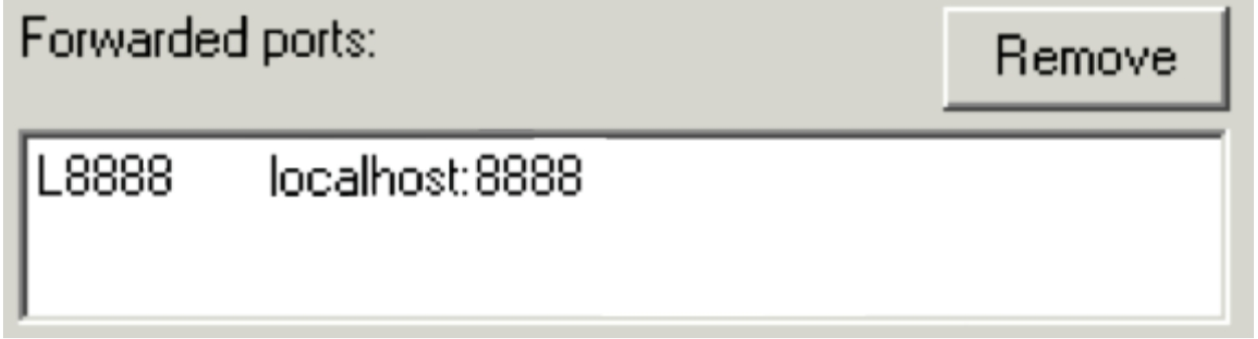
\includegraphics{./images/forward_ports.png}

\begin{enumerate}
\def\labelenumi{\arabic{enumi}.}
\setcounter{enumi}{73}
\tightlist
\item
  Click \textbf{Open} to start the session.
\item
  If prompted to cache the server's host key, click \textbf{Yes}. If the connection is not successful, the instance might still be launching. Wait two minutes then try connecting again by clicking the PuTTY icon in the top-left corner of the PuTTY window and selecting \textbf{Restart session}. If you are prompted for a username, type: ec2-usera.
\end{enumerate}

\hypertarget{connect-to-your-deep-learning-ami-instance-from-a-mac-or-linux-machine}{%
\section{Connect to Your Deep Learning AMI Instance from a Mac or Linux Machine}\label{connect-to-your-deep-learning-ami-instance-from-a-mac-or-linux-machine}}

\begin{enumerate}
\def\labelenumi{\arabic{enumi}.}
\setcounter{enumi}{75}
\tightlist
\item
  Start a new \textbf{Terminal} session on your computer.
\item
  Run the following command, replacing \textbf{PATH-TO-PEM.pem} with your *\textbf{.PEM} key path:
\end{enumerate}

\begin{Shaded}
\begin{Highlighting}[]
\NormalTok{chmod }\DecValTok{400}\NormalTok{ PATH}\OperatorTok{-}\NormalTok{TO}\OperatorTok{-}\NormalTok{PEM.pem }
\end{Highlighting}
\end{Shaded}

Example:

\begin{Shaded}
\begin{Highlighting}[]
\NormalTok{chmod }\DecValTok{400} \OperatorTok{/}\NormalTok{keys}\OperatorTok{/}\NormalTok{qwiklabs1234.pem }
\end{Highlighting}
\end{Shaded}

\begin{enumerate}
\def\labelenumi{\arabic{enumi}.}
\setcounter{enumi}{77}
\tightlist
\item
  Run the following command, replacing the \textbf{PATH-TO-PEM.pem} with your *\textbf{.PEM} key and replacing \textbf{YOUR-IP-ADDRESS} with the \textbf{instance IP address} you copied earlier:
\end{enumerate}

\begin{Shaded}
\begin{Highlighting}[]
\NormalTok{ssh }\OperatorTok{-}\NormalTok{i PATH}\OperatorTok{-}\NormalTok{TO}\OperatorTok{-}\NormalTok{PEM.pem }\OperatorTok{-}\NormalTok{L }\DecValTok{8888}\OperatorTok{:}\NormalTok{localhost}\OperatorTok{:}\DecValTok{8888} 
\NormalTok{ec2}\OperatorTok{-}\NormalTok{user}\OperatorTok{@}\NormalTok{YOUR}\OperatorTok{-}\NormalTok{IP}\OperatorTok{-}\NormalTok{ADDRESS }
\end{Highlighting}
\end{Shaded}

For example:

\begin{Shaded}
\begin{Highlighting}[]
\NormalTok{ssh }\OperatorTok{-}\NormalTok{i }\OperatorTok{/}\NormalTok{keys}\OperatorTok{/}\NormalTok{qwikLABS}\OperatorTok{-}\NormalTok{L1234}\FloatTok{-12345.}\NormalTok{pem }\OperatorTok{-}\NormalTok{L }\DecValTok{8888}\OperatorTok{:}\NormalTok{localhost}\OperatorTok{:}\DecValTok{8888} 
\NormalTok{ec2}\OperatorTok{-}\NormalTok{user}\OperatorTok{@}\DecValTok{11}\NormalTok{.}\DecValTok{22}\NormalTok{.}\FloatTok{33.44}
\end{Highlighting}
\end{Shaded}

\begin{enumerate}
\def\labelenumi{\arabic{enumi}.}
\setcounter{enumi}{78}
\tightlist
\item
  If prompted to continue connecting, type: yes.
\end{enumerate}

\hypertarget{explore-amazon-deep-learning-ami-and-connect-to-a-jupyter-notebook}{%
\chapter{Explore Amazon Deep Learning AMI and Connect to a Jupyter Notebook}\label{explore-amazon-deep-learning-ami-and-connect-to-a-jupyter-notebook}}

Jupyter notebooks are documents that allow you to create and share documents that contain both code as well as rich text elements such as equations. If you are unfamiliar with Jupyter notebooks, see Jupyter notebook docs online.\\
80. In your SSH session, you will find various deep learning frameworks like MXNet, TensorFlow, Keras as well as Anaconda installed on the deep learning AMI.\\
81. Type \texttt{source\ activate\ tensorflow\_p36} (you could choose the framework you want to activate) in your SSH session.\\
82. Type \texttt{nvidia-smi\ -L} to check the availability of GPU on the instance. Your EC2 instance has a Nvidia GPU processor.\\
83. To start a Jupyter notebook, type \texttt{nohup\ jupyter\ notebook\ -\/-no-browser\ \&}\\
Press \textbf{Enter} if the command-line hangs while running.\\
84. To view the output of the previous command, type \texttt{tail\ nohup.out}.\\
You should see a message like this: \texttt{Copy/paste\ this\ URL\ into\ your\ browser} when you connect for the first time, to login with a token: \texttt{http://localhost:8888/?token=xxxx}.\\
If you did not see this output, wait 30 seconds and run the command again until it appears.\\
85. \textbf{Copy} the URL from the terminal and \textbf{paste} it into a new web browser tab.\\
86. You should see the following page (or similar page):

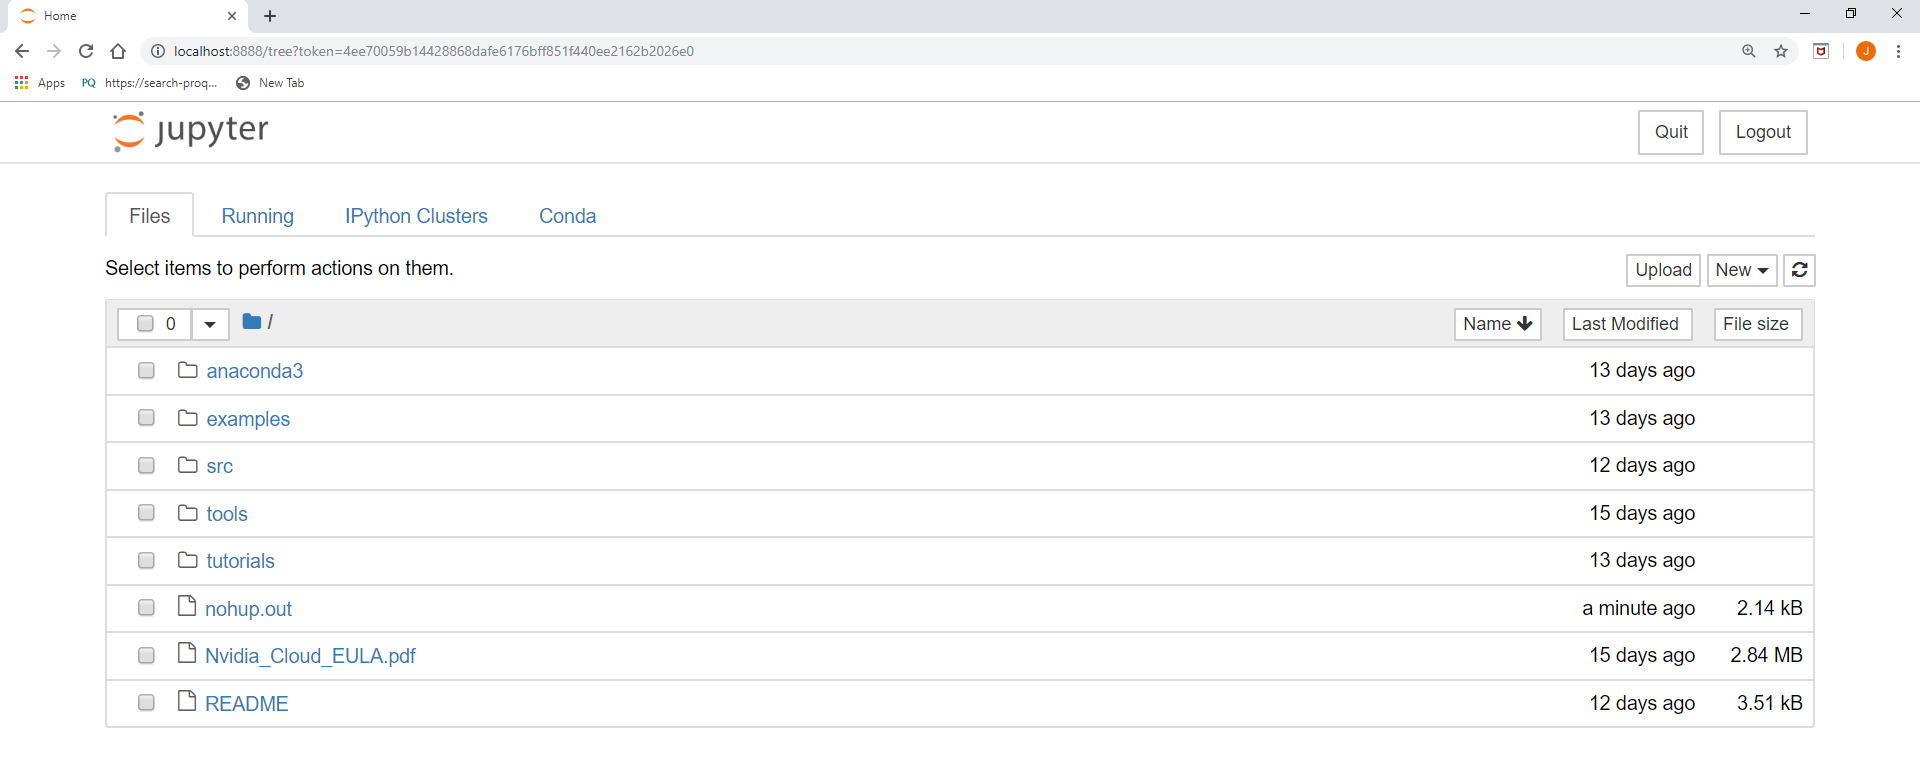
\includegraphics{./images/jupyter.png}

It might take a minute for the notebook page to appear. Give it time to fully load.\\
87. To create a Jupyter notebook, click \textbf{New}, then click \textbf{Python3}. A new tab will open that will display a Jupyter Notebook. You will next create a deep learning model in this notebook.

\hypertarget{create-and-run-a-multi-layer-perceptron-model-using-neural-networks}{%
\chapter{Create and Run a Multi-Layer Perceptron Model Using Neural Networks}\label{create-and-run-a-multi-layer-perceptron-model-using-neural-networks}}

The example below uses some basic functions from TensorFlow to create neural networks over the customized data sets stored in S3 and write the result plots to S3. The example uses AWID wireless network intrusion detection dataset with 154 features and a class label having 4 network activity type categories. The data set has been pre-processed with data transformation, normalization, and under-sampling.

\hypertarget{install-and-import-dependencies}{%
\section{Install and Import Dependencies}\label{install-and-import-dependencies}}

\begin{enumerate}
\def\labelenumi{\arabic{enumi}.}
\setcounter{enumi}{87}
\tightlist
\item
  Paste the following code into the \textbf{In} cell in the jupyter notebook to \textbf{import dependencies} into the notebook cell:
\end{enumerate}

\begin{Shaded}
\begin{Highlighting}[]
\ImportTok{import}\NormalTok{ pandas }\ImportTok{as}\NormalTok{ pd}
\ImportTok{import}\NormalTok{ numpy }\ImportTok{as}\NormalTok{ np}
\ImportTok{import}\NormalTok{ tensorflow }\ImportTok{as}\NormalTok{ tf}
\ImportTok{import}\NormalTok{ datetime}
\ImportTok{import}\NormalTok{ matplotlib.pyplot }\ImportTok{as}\NormalTok{ plt}
\ImportTok{from}\NormalTok{ sklearn.utils }\ImportTok{import}\NormalTok{ shuffle}
\ImportTok{from}\NormalTok{ smart_open }\ImportTok{import} \BuiltInTok{open}
\end{Highlighting}
\end{Shaded}

\begin{enumerate}
\def\labelenumi{\arabic{enumi}.}
\setcounter{enumi}{88}
\tightlist
\item
  \textbf{smart\_open} is a Python 2 \& Python 3 library for efficient streaming of very large files from/to storages such as S3, HDFS, WebHDFS, HTTP, HTTPS, SFTP, or local filesystem. It builds on boto3 and other remote storage libraries but offers a clean unified Pythonic API. Unlike the other packages in the example, you need to \textbf{install this package} to the ``tensorflow\_p36'' environment before you can import it in the code. To do that, go to jupyter \textbf{Home} tab, click \textbf{Conda}. Remember we have activated the ``tensorflow\_p36'' environment.
\item
  Select the ``\textbf{smart\_open}'' package in the left bottom plane and move it to the right bottom plane by clicking the \textbf{arrow} button.
\item
  You should see the ``smart\_open'' package show up in the right bottom plane. Click \textbf{Refresh package list}.
\item
  \textbf{Repeat} the steps 80-87 to make sure that the installed packages in the ``tensorflow\_p36'' environment are fully updated.
\item
  Run the cell by pressing \textbf{Shift+Enter} or click on \textbf{Run}. When the cell finishes running, the number on the left of the cell will change from \textbf{In{[}*{]}:} to \textbf{In{[}1{]}}.
\end{enumerate}

\hypertarget{provide-utilities-related-functions}{%
\section{Provide Utilities-Related Functions}\label{provide-utilities-related-functions}}

\begin{enumerate}
\def\labelenumi{\arabic{enumi}.}
\setcounter{enumi}{93}
\tightlist
\item
  Provide the \textbf{utilities functions} for reading files, checking column names, checking missing values, and transforming the class labels from a categorical variable to 4 dummy variables.
\end{enumerate}

\begin{Shaded}
\begin{Highlighting}[]
\CommentTok{# Utilities-related functions}
\KeywordTok{def}\NormalTok{ now():}
\NormalTok{    tmp }\OperatorTok{=}\NormalTok{ datetime.datetime.now().strftime(}\StringTok{"%Y-%m-}\SpecialCharTok{%d}\StringTok{ %H:%M:%S"}\NormalTok{)}
    \ControlFlowTok{return}\NormalTok{ tmp}

\KeywordTok{def}\NormalTok{ read_file(}\BuiltInTok{file}\NormalTok{):}
    \ControlFlowTok{try}\NormalTok{:}
\NormalTok{        df }\OperatorTok{=}\NormalTok{ pd.read_csv(}\BuiltInTok{file}\NormalTok{, index_col }\OperatorTok{=} \DecValTok{0}\NormalTok{)}
        \BuiltInTok{print}\NormalTok{(}\StringTok{"}\SpecialCharTok{\{\}}\StringTok{: }\SpecialCharTok{\{\}}\StringTok{ has }\SpecialCharTok{\{\}}\StringTok{ observations and }\SpecialCharTok{\{\}}\StringTok{ columns"}\NormalTok{.}\BuiltInTok{format}\NormalTok{(now(), }\BuiltInTok{file}\NormalTok{, df.shape[}\DecValTok{0}\NormalTok{], df.shape[}\DecValTok{1}\NormalTok{]))}
        \BuiltInTok{print}\NormalTok{(}\StringTok{"}\SpecialCharTok{\{\}}\StringTok{: Column name checking::: }\SpecialCharTok{\{\}}\StringTok{"}\NormalTok{.}\BuiltInTok{format}\NormalTok{(now(), df.columns.tolist()))}
    \ControlFlowTok{except} \PreprocessorTok{MemoryError} \ImportTok{as}\NormalTok{ e:}
        \BuiltInTok{print}\NormalTok{(e.message)}
    \ControlFlowTok{return}\NormalTok{ df}

\CommentTok{# Read data frame, check missing data, find number of missing}
\KeywordTok{def}\NormalTok{ check_missing(df):}
    \ControlFlowTok{try}\NormalTok{:}
        \ControlFlowTok{if}\NormalTok{(}\BuiltInTok{isinstance}\NormalTok{(df, pd.DataFrame)):}
\NormalTok{            na_pool }\OperatorTok{=}\NormalTok{ pd.concat([df.isnull().}\BuiltInTok{any}\NormalTok{(), df.isnull().}\BuiltInTok{sum}\NormalTok{(), df.isnull().}\BuiltInTok{sum}\NormalTok{() }\OperatorTok{/}\NormalTok{ df.shape[}\DecValTok{0}\NormalTok{]], axis }\OperatorTok{=} \DecValTok{1}\NormalTok{, keys }\OperatorTok{=}\NormalTok{ [}\StringTok{"na_bool"}\NormalTok{, }\StringTok{"na_sum"}\NormalTok{, }\StringTok{"na_percent"}\NormalTok{])}
\NormalTok{            na_pool }\OperatorTok{=}\NormalTok{ na_pool.loc[na_pool[}\StringTok{"na_bool"}\NormalTok{] }\OperatorTok{==}  \VariableTok{True}\NormalTok{]}
            \ControlFlowTok{return}\NormalTok{ na_pool}
        \ControlFlowTok{else}\NormalTok{:}
            \BuiltInTok{print}\NormalTok{(}\StringTok{"}\SpecialCharTok{\{\}}\StringTok{: The input is not panda DataFrame"}\NormalTok{.}\BuiltInTok{format}\NormalTok{(now()))}
    \ControlFlowTok{except}\NormalTok{ (}\PreprocessorTok{UnboundLocalError}\NormalTok{, }\PreprocessorTok{RuntimeError}\NormalTok{):}
        \BuiltInTok{print}\NormalTok{(}\StringTok{"}\SpecialCharTok{\{\}}\StringTok{: The input has something wrong"}\NormalTok{.}\BuiltInTok{format}\NormalTok{(now()))}

\KeywordTok{def}\NormalTok{ transform(df):}
\NormalTok{    df.loc[df.}\BuiltInTok{type} \OperatorTok{==} \DecValTok{1}\NormalTok{, }\StringTok{'isNormal'}\NormalTok{] }\OperatorTok{=} \DecValTok{1}
\NormalTok{    df.loc[df.}\BuiltInTok{type} \OperatorTok{!=} \DecValTok{1}\NormalTok{, }\StringTok{'isNormal'}\NormalTok{] }\OperatorTok{=} \DecValTok{0}

\NormalTok{    df.loc[df.}\BuiltInTok{type} \OperatorTok{==} \DecValTok{2}\NormalTok{, }\StringTok{'isImpersonation'}\NormalTok{] }\OperatorTok{=} \DecValTok{1}
\NormalTok{    df.loc[df.}\BuiltInTok{type} \OperatorTok{!=} \DecValTok{2}\NormalTok{, }\StringTok{'isImpersonation'}\NormalTok{] }\OperatorTok{=} \DecValTok{0}

\NormalTok{    df.loc[df.}\BuiltInTok{type} \OperatorTok{==} \DecValTok{3}\NormalTok{, }\StringTok{'isFlooding'}\NormalTok{] }\OperatorTok{=} \DecValTok{1}
\NormalTok{    df.loc[df.}\BuiltInTok{type} \OperatorTok{!=} \DecValTok{3}\NormalTok{, }\StringTok{'isFlooding'}\NormalTok{] }\OperatorTok{=} \DecValTok{0}

\NormalTok{    df.loc[df.}\BuiltInTok{type} \OperatorTok{==} \DecValTok{4}\NormalTok{, }\StringTok{'isInjection'}\NormalTok{] }\OperatorTok{=} \DecValTok{1}
\NormalTok{    df.loc[df.}\BuiltInTok{type} \OperatorTok{!=} \DecValTok{4}\NormalTok{, }\StringTok{'isInjection'}\NormalTok{] }\OperatorTok{=} \DecValTok{0}

    \BuiltInTok{print}\NormalTok{(df.isNormal.value_counts())}
    \BuiltInTok{print}\NormalTok{(df.isImpersonation.value_counts())}
    \BuiltInTok{print}\NormalTok{(df.isFlooding.value_counts())}
    \BuiltInTok{print}\NormalTok{(df.isInjection.value_counts())}

\NormalTok{    df2 }\OperatorTok{=}\NormalTok{ pd.concat([df.isNormal, df.isImpersonation, df.isFlooding, df.isInjection], axis }\OperatorTok{=} \DecValTok{1}\NormalTok{)}
\NormalTok{    df1 }\OperatorTok{=}\NormalTok{ df.drop([}\StringTok{'type'}\NormalTok{, }\StringTok{'isNormal'}\NormalTok{, }\StringTok{'isImpersonation'}\NormalTok{, }\StringTok{'isFlooding'}\NormalTok{, }\StringTok{'isInjection'}\NormalTok{], axis }\OperatorTok{=} \DecValTok{1}\NormalTok{)   }

    \ControlFlowTok{return}\NormalTok{ df1, df2}
\end{Highlighting}
\end{Shaded}

\hypertarget{read-data-from-s3-and-inspect-the-data}{%
\section{Read Data from S3 and Inspect the Data}\label{read-data-from-s3-and-inspect-the-data}}

\begin{enumerate}
\def\labelenumi{\arabic{enumi}.}
\setcounter{enumi}{94}
\tightlist
\item
  You need to find the \textbf{Access Key} and the \textbf{Secret Access Key}. Click on your \textbf{username} at the top right of the AWS Management Console page.
\item
  Click on the \textbf{My Security Credentials} link from the drop-down menu.
\item
  Find the \textbf{Access keys (access key ID and secret access key)} section and click on \textbf{Create New Access Key}.
\item
  Download the \textbf{Access Key file (in .csv format)} to a safe local folder for later use.
\item
  Paste the following code into the \textbf{In} cell in the jupyter notebook to read data (both training set and testing set) from S3 and then inspect the data:
\end{enumerate}

\begin{Shaded}
\begin{Highlighting}[]
\CommentTok{# Read in datafile}
\NormalTok{aws_key }\OperatorTok{=} \StringTok{'YOUR_AWS_ACCESS_KEY'}
\NormalTok{aws_secret }\OperatorTok{=} \StringTok{'YOUR_AWS_SECRET_ACCESS_KEY'}

\NormalTok{bucket_name }\OperatorTok{=} \StringTok{'YOUR_S3_BUCKET_NAME'}
\NormalTok{object_train_key }\OperatorTok{=} \StringTok{'train.csv'}
\NormalTok{object_test_key }\OperatorTok{=} \StringTok{'test.csv'}

\NormalTok{path_train }\OperatorTok{=} \StringTok{'s3://}\SpecialCharTok{\{\}}\StringTok{:}\SpecialCharTok{\{\}}\StringTok{@}\SpecialCharTok{\{\}}\StringTok{/}\SpecialCharTok{\{\}}\StringTok{'}\NormalTok{.}\BuiltInTok{format}\NormalTok{(aws_key, aws_secret, bucket_name, object_train_key)}
\NormalTok{path_test }\OperatorTok{=} \StringTok{'s3://}\SpecialCharTok{\{\}}\StringTok{:}\SpecialCharTok{\{\}}\StringTok{@}\SpecialCharTok{\{\}}\StringTok{/}\SpecialCharTok{\{\}}\StringTok{'}\NormalTok{.}\BuiltInTok{format}\NormalTok{(aws_key, aws_secret, bucket_name, object_test_key)}

\NormalTok{data_trn }\OperatorTok{=}\NormalTok{ read_file(smart_open(path_train))}
\BuiltInTok{print}\NormalTok{(check_missing(data_trn))}
\NormalTok{data_trn.rename(columns}\OperatorTok{=}\NormalTok{\{}\StringTok{'154'}\NormalTok{:}\StringTok{'type'}\NormalTok{\}, inplace}\OperatorTok{=}\VariableTok{True}\NormalTok{)}
\BuiltInTok{print}\NormalTok{(data_trn.head(}\DecValTok{5}\NormalTok{))}
\BuiltInTok{print}\NormalTok{(data_trn.}\BuiltInTok{type}\NormalTok{.value_counts())}

\NormalTok{data_tst }\OperatorTok{=}\NormalTok{ read_file(smart_open(path_test))}
\BuiltInTok{print}\NormalTok{(check_missing(data_tst))}
\NormalTok{data_tst.rename(columns}\OperatorTok{=}\NormalTok{\{}\StringTok{'154'}\NormalTok{:}\StringTok{'type'}\NormalTok{\}, inplace}\OperatorTok{=}\VariableTok{True}\NormalTok{)}
\BuiltInTok{print}\NormalTok{(data_tst.head(}\DecValTok{5}\NormalTok{))}
\BuiltInTok{print}\NormalTok{(data_tst.}\BuiltInTok{type}\NormalTok{.value_counts())}
\end{Highlighting}
\end{Shaded}

\hypertarget{perform-the-data-processing-specific-to-neural-networks}{%
\section{Perform the Data Processing Specific to Neural Networks}\label{perform-the-data-processing-specific-to-neural-networks}}

\begin{enumerate}
\def\labelenumi{\arabic{enumi}.}
\setcounter{enumi}{99}
\tightlist
\item
  Split the \textbf{training set} into a \textbf{training part} and a \textbf{validation part}:
\end{enumerate}

\begin{Shaded}
\begin{Highlighting}[]
\NormalTok{normal }\OperatorTok{=}\NormalTok{ data_trn[data_trn.}\BuiltInTok{type} \OperatorTok{==} \DecValTok{1}\NormalTok{]}
\NormalTok{impersonation }\OperatorTok{=}\NormalTok{ data_trn[data_trn.}\BuiltInTok{type} \OperatorTok{==} \DecValTok{2}\NormalTok{]}
\NormalTok{flooding }\OperatorTok{=}\NormalTok{ data_trn[data_trn.}\BuiltInTok{type} \OperatorTok{==} \DecValTok{3}\NormalTok{]}
\NormalTok{injection }\OperatorTok{=}\NormalTok{ data_trn[data_trn.}\BuiltInTok{type} \OperatorTok{==} \DecValTok{4}\NormalTok{]}

\NormalTok{normal_trn }\OperatorTok{=}\NormalTok{ normal.sample(frac }\OperatorTok{=} \FloatTok{0.7}\NormalTok{)}
\NormalTok{impersonation_trn }\OperatorTok{=}\NormalTok{ impersonation.sample(frac }\OperatorTok{=} \FloatTok{0.7}\NormalTok{)}
\NormalTok{flooding_trn }\OperatorTok{=}\NormalTok{ flooding.sample(frac }\OperatorTok{=} \FloatTok{0.7}\NormalTok{)}
\NormalTok{injection_trn }\OperatorTok{=}\NormalTok{ injection.sample(frac }\OperatorTok{=} \FloatTok{0.7}\NormalTok{)}
\NormalTok{train }\OperatorTok{=}\NormalTok{ pd.concat([normal_trn, impersonation_trn, flooding_trn, injection_trn], axis }\OperatorTok{=} \DecValTok{0}\NormalTok{)}
\NormalTok{validation }\OperatorTok{=}\NormalTok{ data_trn.loc[}\OperatorTok{~}\NormalTok{data_trn.index.isin(train.index)]}

\CommentTok{#shuffle the dataframes so that rows are in random order}
\NormalTok{train }\OperatorTok{=}\NormalTok{ shuffle(train)}
\NormalTok{validation }\OperatorTok{=}\NormalTok{ shuffle(validation)}
\end{Highlighting}
\end{Shaded}

\begin{enumerate}
\def\labelenumi{\arabic{enumi}.}
\setcounter{enumi}{100}
\tightlist
\item
  \textbf{Transform the class labels} from a categorical variable to 4 dummy variables and \textbf{check} the correctness:
\end{enumerate}

\begin{Shaded}
\begin{Highlighting}[]
\NormalTok{x_train, y_train }\OperatorTok{=}\NormalTok{ transform(train)}
\NormalTok{x_validation, y_validation }\OperatorTok{=}\NormalTok{ transform(validation)}
\NormalTok{x_test, y_test }\OperatorTok{=}\NormalTok{ transform(data_tst)}

 \CommentTok{# check to ensure that all of training and testing sets have correct shape}
\BuiltInTok{print}\NormalTok{(x_train.shape)}
\BuiltInTok{print}\NormalTok{(y_train.shape)}
\BuiltInTok{print}\NormalTok{(x_validation.shape)}
\BuiltInTok{print}\NormalTok{(y_validation.shape)  }
\BuiltInTok{print}\NormalTok{(x_test.shape)}
\BuiltInTok{print}\NormalTok{(y_test.shape)  }
\end{Highlighting}
\end{Shaded}

\hypertarget{create-a-multi-layer-perceptron-model-using-neural-networks}{%
\section{Create a Multi-Layer Perceptron Model Using Neural Networks}\label{create-a-multi-layer-perceptron-model-using-neural-networks}}

\begin{enumerate}
\def\labelenumi{\arabic{enumi}.}
\setcounter{enumi}{101}
\tightlist
\item
  Define \textbf{parameters} for your neural network:
\end{enumerate}

\begin{Shaded}
\begin{Highlighting}[]
\CommentTok{# parameters}
\NormalTok{learning_rate }\OperatorTok{=} \FloatTok{0.005}
\NormalTok{data_size }\OperatorTok{=}\NormalTok{ x_train.shape[}\DecValTok{0}\NormalTok{]}
\NormalTok{batch_size }\OperatorTok{=} \DecValTok{1150}
\NormalTok{training_epochs }\OperatorTok{=} \DecValTok{2000}
\NormalTok{training_dropout }\OperatorTok{=} \FloatTok{0.9}
\end{Highlighting}
\end{Shaded}

\begin{enumerate}
\def\labelenumi{\arabic{enumi}.}
\setcounter{enumi}{102}
\tightlist
\item
  Define the \textbf{neural network configuration}:
\end{enumerate}

\begin{Shaded}
\begin{Highlighting}[]
\CommentTok{# input place holders}
\NormalTok{x }\OperatorTok{=}\NormalTok{ tf.compat.v1.placeholder(tf.float32, [}\VariableTok{None}\NormalTok{, x_train.shape[}\DecValTok{1}\NormalTok{]])}
\NormalTok{y }\OperatorTok{=}\NormalTok{ tf.compat.v1.placeholder(tf.float32, [}\VariableTok{None}\NormalTok{, y_train.shape[}\DecValTok{1}\NormalTok{]])}
\NormalTok{rate }\OperatorTok{=}\NormalTok{ tf.compat.v1.placeholder(tf.float32)}

\CommentTok{#weights, bias, and activation function for n layers}
\NormalTok{num_nodes }\OperatorTok{=} \BuiltInTok{int}\NormalTok{(x_train.shape[}\DecValTok{1}\NormalTok{] }\OperatorTok{*}\NormalTok{ (}\DecValTok{2} \OperatorTok{/} \DecValTok{3}\NormalTok{))}
\NormalTok{w1 }\OperatorTok{=}\NormalTok{ tf.Variable(tf.random.normal([x_train.shape[}\DecValTok{1}\NormalTok{], num_nodes], stddev }\OperatorTok{=} \FloatTok{0.15}\NormalTok{))}
\NormalTok{b1 }\OperatorTok{=}\NormalTok{ tf.Variable(tf.random.normal([num_nodes]))}
\NormalTok{a1 }\OperatorTok{=}\NormalTok{ tf.nn.relu(tf.matmul(x, w1) }\OperatorTok{+}\NormalTok{ b1)}
\NormalTok{a1_out }\OperatorTok{=}\NormalTok{ tf.nn.dropout(a1, rate }\OperatorTok{=}\NormalTok{ rate)}

\NormalTok{w2 }\OperatorTok{=}\NormalTok{ tf.Variable(tf.random.normal([num_nodes, y_train.shape[}\DecValTok{1}\NormalTok{]], stddev }\OperatorTok{=} \FloatTok{0.15}\NormalTok{))}
\NormalTok{b2 }\OperatorTok{=}\NormalTok{ tf.Variable(tf.random.normal([y_train.shape[}\DecValTok{1}\NormalTok{]]))}
\NormalTok{z2 }\OperatorTok{=}\NormalTok{ tf.matmul(a1_out, w2) }\OperatorTok{+}\NormalTok{ b2}
\NormalTok{a2 }\OperatorTok{=}\NormalTok{ tf.nn.softmax(z2)}
\end{Highlighting}
\end{Shaded}

If you define a multi-layer network with linear neurons, then the network will only be a linear function. To allow the network to capture non-linear properties, you can add an activation function at each layer. The activation functions could be ReLU, sigmoid, or tanh.\\
104. Define a \textbf{cost function} and an \textbf{optimizer} to learn the \textbf{weights} and \textbf{biases}:

\begin{Shaded}
\begin{Highlighting}[]
\NormalTok{cost }\OperatorTok{=}\NormalTok{ tf.reduce_mean(tf.nn.softmax_cross_entropy_with_logits_v2(logits }\OperatorTok{=}\NormalTok{ z2, labels }\OperatorTok{=}\NormalTok{ y))}
\NormalTok{optimizer }\OperatorTok{=}\NormalTok{ tf.compat.v1.train.AdamOptimizer(learning_rate }\OperatorTok{=}\NormalTok{ learning_rate).minimize(cost)}
\end{Highlighting}
\end{Shaded}

\begin{enumerate}
\def\labelenumi{\arabic{enumi}.}
\setcounter{enumi}{104}
\tightlist
\item
  Define the \textbf{evaluation metric}:
\end{enumerate}

\begin{Shaded}
\begin{Highlighting}[]
\NormalTok{pred }\OperatorTok{=}\NormalTok{ tf.argmax(a2, }\DecValTok{1}\NormalTok{)}
\NormalTok{correct }\OperatorTok{=}\NormalTok{ tf.equal(tf.argmax(a2, }\DecValTok{1}\NormalTok{), tf.argmax(y, }\DecValTok{1}\NormalTok{))}
\NormalTok{accuracy }\OperatorTok{=}\NormalTok{ tf.reduce_mean(tf.cast(correct, tf.float32))}
\end{Highlighting}
\end{Shaded}

\hypertarget{train-the-multi-layer-perceptron-model}{%
\section{Train the Multi-Layer Perceptron Model}\label{train-the-multi-layer-perceptron-model}}

\begin{enumerate}
\def\labelenumi{\arabic{enumi}.}
\setcounter{enumi}{105}
\tightlist
\item
  Set up the \textbf{data structures} and \textbf{file paths} to \textbf{save the intermediate training results}:
\end{enumerate}

\begin{Shaded}
\begin{Highlighting}[]
\CommentTok{# train model}
\NormalTok{train_accuracy_summary }\OperatorTok{=}\NormalTok{ []}
\NormalTok{train_cost_summary }\OperatorTok{=}\NormalTok{ []}
\NormalTok{valid_accuracy_summary }\OperatorTok{=}\NormalTok{ []}
\NormalTok{valid_cost_summary }\OperatorTok{=}\NormalTok{ []}
\NormalTok{stop_early }\OperatorTok{=} \DecValTok{0}

\NormalTok{checkpoint1 }\OperatorTok{=} \StringTok{'./best_model_pca.ckpt'}
\NormalTok{checkpoint2 }\OperatorTok{=} \StringTok{'./weights_pca.ckpt'}
\NormalTok{saver }\OperatorTok{=}\NormalTok{ tf.compat.v1.train.Saver(max_to_keep }\OperatorTok{=} \DecValTok{1}\NormalTok{)}
\NormalTok{weights_saver }\OperatorTok{=}\NormalTok{ tf.compat.v1.train.Saver(var_list }\OperatorTok{=}\NormalTok{ [w1])}
\end{Highlighting}
\end{Shaded}

We use the \textbf{temporary storage} associated with this EC2 Deep Learning instance to save the intermediate training results. Those results will be gone when the instance is terminated. It is not efficient to save those intermediate results to S3. Since the instance is run on Amazon Linux system (instead of Windows), please make sure to write down the correct file paths.\\
107. Run the \textbf{training loop} with the defined parameters in step 102. We save the model and its associated weights only for the model with the highest validation accuracy. We also use an early stop criterion to stop the training loop early if the model has been trained long enough and the validation accuracy cannot be improved further in the next 20 loops.

\begin{Shaded}
\begin{Highlighting}[]
\ControlFlowTok{with}\NormalTok{ tf.compat.v1.Session() }\ImportTok{as}\NormalTok{ sess:}
\NormalTok{    sess.run(tf.compat.v1.global_variables_initializer())}

    \ControlFlowTok{for}\NormalTok{ epoch }\KeywordTok{in} \BuiltInTok{range}\NormalTok{(training_epochs):}
        \ControlFlowTok{for}\NormalTok{ batch }\KeywordTok{in} \BuiltInTok{range}\NormalTok{(}\BuiltInTok{int}\NormalTok{(data_size}\OperatorTok{/}\NormalTok{batch_size)):}
\NormalTok{            batch_x }\OperatorTok{=}\NormalTok{ x_train[batch}\OperatorTok{*}\NormalTok{batch_size: (}\DecValTok{1}\OperatorTok{+}\NormalTok{batch)}\OperatorTok{*}\NormalTok{batch_size]}
\NormalTok{            batch_y }\OperatorTok{=}\NormalTok{ y_train[batch}\OperatorTok{*}\NormalTok{batch_size: (}\DecValTok{1}\OperatorTok{+}\NormalTok{batch)}\OperatorTok{*}\NormalTok{batch_size]}

\NormalTok{            sess.run([optimizer], feed_dict }\OperatorTok{=}\NormalTok{ \{x: batch_x, y: batch_y, rate: }\DecValTok{1} \OperatorTok{-}\NormalTok{ training_dropout\})}

\NormalTok{        train_accuracy, train_cost }\OperatorTok{=}\NormalTok{ sess.run([accuracy, cost], feed_dict }\OperatorTok{=}\NormalTok{ \{x: x_train, y: y_train, rate: }\DecValTok{1} \OperatorTok{-}\NormalTok{ training_dropout\})}
\NormalTok{        valid_accuracy, valid_cost }\OperatorTok{=}\NormalTok{ sess.run([accuracy, cost], feed_dict }\OperatorTok{=}\NormalTok{ \{x: x_validation, y: y_validation, rate: }\DecValTok{1} \OperatorTok{-}\NormalTok{ training_dropout\})}

        \BuiltInTok{print}\NormalTok{(}\StringTok{"Epoch:"}\NormalTok{, epoch,}
              \StringTok{"Train_Accuracy ="}\NormalTok{, }\StringTok{"}\SpecialCharTok{\{:.5f\}}\StringTok{"}\NormalTok{.}\BuiltInTok{format}\NormalTok{(train_accuracy),}
              \StringTok{"Train_Cost ="}\NormalTok{, }\StringTok{"}\SpecialCharTok{\{:.5f\}}\StringTok{"}\NormalTok{.}\BuiltInTok{format}\NormalTok{(train_cost), }
              \StringTok{"Valid_Accuracy ="}\NormalTok{, }\StringTok{"}\SpecialCharTok{\{:.5f\}}\StringTok{"}\NormalTok{.}\BuiltInTok{format}\NormalTok{(valid_accuracy),}
              \StringTok{"Valid_Cost ="}\NormalTok{, }\StringTok{"}\SpecialCharTok{\{:.5f\}}\StringTok{"}\NormalTok{.}\BuiltInTok{format}\NormalTok{(valid_cost))}

        \ControlFlowTok{if}\NormalTok{ epoch }\OperatorTok{>} \DecValTok{0} \KeywordTok{and}\NormalTok{ valid_accuracy }\OperatorTok{>} \BuiltInTok{max}\NormalTok{(valid_accuracy_summary):}
\NormalTok{            saver.save(sess, checkpoint1)}
\NormalTok{            weights_saver.save(sess, checkpoint2)}

\NormalTok{        train_accuracy_summary.append(train_accuracy)}
\NormalTok{        train_cost_summary.append(train_cost)}
\NormalTok{        valid_accuracy_summary.append(valid_accuracy)}
\NormalTok{        valid_cost_summary.append(valid_cost)}
       
        \ControlFlowTok{if}\NormalTok{ valid_accuracy }\OperatorTok{<} \BuiltInTok{max}\NormalTok{(valid_accuracy_summary) }\KeywordTok{and}\NormalTok{ epoch }\OperatorTok{>} \DecValTok{1000}\NormalTok{:}
\NormalTok{            stop_early }\OperatorTok{+=} \DecValTok{1}
            \ControlFlowTok{if}\NormalTok{ stop_early }\OperatorTok{==} \DecValTok{20}\NormalTok{:}
                \ControlFlowTok{break}
        \ControlFlowTok{else}\NormalTok{:}
\NormalTok{            stop_early }\OperatorTok{=} \DecValTok{0}

    \BuiltInTok{print}\NormalTok{()}
    \BuiltInTok{print}\NormalTok{(}\StringTok{"Optimization Finished!"}\NormalTok{)}
\end{Highlighting}
\end{Shaded}

\hypertarget{evaluate-the-multi-layer-perceptron-model}{%
\section{Evaluate the Multi-Layer Perceptron Model}\label{evaluate-the-multi-layer-perceptron-model}}

\begin{enumerate}
\def\labelenumi{\arabic{enumi}.}
\setcounter{enumi}{107}
\tightlist
\item
  We restore the \textbf{best model} saved from the training phase and run this model on the \textbf{test set} to get the testing accuracy.
\item
  We also restore the \textbf{weights} associated with the best model and then use them to calculate the \textbf{importance score for each feature} and print the scores out in the descending order.
\item
  We plot the feature importance and \textbf{save the plot permanently to S3} using the ``\textbf{smart\_open}'' Python library. The following code covers the steps 108-110.
\end{enumerate}

\begin{Shaded}
\begin{Highlighting}[]
\ControlFlowTok{with}\NormalTok{ tf.compat.v1.Session() }\ImportTok{as}\NormalTok{ sess:}
\NormalTok{    saver.restore(sess, checkpoint1)}
\NormalTok{    weights_saver.restore(sess, checkpoint2)}
\NormalTok{    graph }\OperatorTok{=}\NormalTok{ tf.compat.v1.get_default_graph()}
    
\NormalTok{    training_accuracy }\OperatorTok{=}\NormalTok{ sess.run(accuracy, feed_dict }\OperatorTok{=}\NormalTok{ \{x: x_train, y: y_train, rate: }\DecValTok{1} \OperatorTok{-}\NormalTok{ training_dropout\})}
\NormalTok{    validation_accuracy }\OperatorTok{=}\NormalTok{ sess.run(accuracy, feed_dict }\OperatorTok{=}\NormalTok{ \{x: x_validation, y: y_validation, rate: }\DecValTok{0}\NormalTok{\})}
    
    \BuiltInTok{print}\NormalTok{(}\StringTok{"Results using the best Validation_Accuracy:"}\NormalTok{)}
    \BuiltInTok{print}\NormalTok{(}\StringTok{"Training Accuracy ="}\NormalTok{, training_accuracy)}
    \BuiltInTok{print}\NormalTok{(}\StringTok{"Validation Accuracy ="}\NormalTok{, validation_accuracy)}

\NormalTok{    testing_prediction, testing_accuracy }\OperatorTok{=}\NormalTok{ sess.run([pred, accuracy], feed_dict }\OperatorTok{=}\NormalTok{ \{x: x_test, y: y_test, rate: }\DecValTok{0}\NormalTok{\})}
    
    \BuiltInTok{print}\NormalTok{()}
    \BuiltInTok{print}\NormalTok{(}\StringTok{"Results using the best Validation_Accuracy:"}\NormalTok{)}
    \BuiltInTok{print}\NormalTok{(}\StringTok{"Testing Accuracy ="}\NormalTok{, testing_accuracy)}

\NormalTok{    w1 }\OperatorTok{=}\NormalTok{ w1.}\BuiltInTok{eval}\NormalTok{(session}\OperatorTok{=}\NormalTok{sess)}
 
\NormalTok{    df }\OperatorTok{=}\NormalTok{ pd.DataFrame(w1)}
    \BuiltInTok{print}\NormalTok{(df.shape)}
    \BuiltInTok{print}\NormalTok{(df.head(}\DecValTok{5}\NormalTok{))}

\NormalTok{    df.loc[:, }\StringTok{"sum"}\NormalTok{] }\OperatorTok{=}\NormalTok{ df.}\BuiltInTok{sum}\NormalTok{(axis }\OperatorTok{=} \DecValTok{1}\NormalTok{)}
    \BuiltInTok{print}\NormalTok{(df.head(}\DecValTok{5}\NormalTok{))}
    

\NormalTok{    dt_importances }\OperatorTok{=} \BuiltInTok{abs}\NormalTok{(df.loc[:, }\StringTok{"sum"}\NormalTok{].values)}
\NormalTok{    dt_indices }\OperatorTok{=}\NormalTok{ np.argsort(dt_importances)[:: }\DecValTok{-1}\NormalTok{]}
    \BuiltInTok{print}\NormalTok{(}\StringTok{"Feature ranking:: ANN:"}\NormalTok{)}

    \ControlFlowTok{for}\NormalTok{ f }\KeywordTok{in} \BuiltInTok{range}\NormalTok{(x_train.shape[}\DecValTok{1}\NormalTok{]):}
        \BuiltInTok{print}\NormalTok{(}\StringTok{"}\SpecialCharTok{%d}\StringTok{. feature }\SpecialCharTok{%d}\StringTok{ importance (}\SpecialCharTok\NormalTok{ (f }\OperatorTok{+} \DecValTok{1}\NormalTok{, dt_indices[f], dt_importances[dt_indices[f]]))}

\NormalTok{    plt.figure()}
\NormalTok{    plt.title(}\StringTok{"Feature importances:: ANN"}\NormalTok{ )}
\NormalTok{    plt.bar(}\BuiltInTok{range}\NormalTok{(x_train.shape[}\DecValTok{1}\NormalTok{]), dt_importances[dt_indices], color }\OperatorTok{=} \StringTok{"r"}\NormalTok{, align }\OperatorTok{=} \StringTok{"center"}\NormalTok{)}
\NormalTok{    plt.xticks(}\BuiltInTok{range}\NormalTok{(x_train.shape[}\DecValTok{1}\NormalTok{]), dt_indices)}
\NormalTok{    plt.xlim([}\OperatorTok{-}\DecValTok{1}\NormalTok{, x_train.shape[}\DecValTok{1}\NormalTok{]])}
\NormalTok{    plt.savefig(}\StringTok{'./importance.png'}\NormalTok{)}

\NormalTok{    importance_key }\OperatorTok{=} \StringTok{'feature_importance.png'}
\NormalTok{    imp_graph_path }\OperatorTok{=} \StringTok{'s3://}\SpecialCharTok{\{\}}\StringTok{:}\SpecialCharTok{\{\}}\StringTok{@}\SpecialCharTok{\{\}}\StringTok{/}\SpecialCharTok{\{\}}\StringTok{'}\NormalTok{.}\BuiltInTok{format}\NormalTok{(aws_key, aws_secret, bucket_name, importance_key)}
    \ControlFlowTok{with} \BuiltInTok{open}\NormalTok{(}\StringTok{'./importance.png'}\NormalTok{, }\StringTok{'rb'}\NormalTok{) }\ImportTok{as}\NormalTok{ f:}
\NormalTok{        content }\OperatorTok{=}\NormalTok{ f.read()}
    \ControlFlowTok{with} \BuiltInTok{open}\NormalTok{(imp_graph_path, }\StringTok{'wb'}\NormalTok{) }\ImportTok{as}\NormalTok{ fout:}
\NormalTok{        fout.write(content)}
\end{Highlighting}
\end{Shaded}

\begin{enumerate}
\def\labelenumi{\arabic{enumi}.}
\setcounter{enumi}{110}
\tightlist
\item
  Finally, we also plot the training vs.~validation accuracy and the training vs.~validation cost over the entire training epochs and \textbf{save the plot permanently to S3} using the ``\textbf{smart\_open}'' Python library.
\end{enumerate}

\begin{Shaded}
\begin{Highlighting}[]
\CommentTok{# Plot accuracy and cost summaries}
\NormalTok{f, (ax1, ax2) }\OperatorTok{=}\NormalTok{ plt.subplots(}\DecValTok{2}\NormalTok{, }\DecValTok{1}\NormalTok{, sharex }\OperatorTok{=} \VariableTok{True}\NormalTok{, figsize }\OperatorTok{=}\NormalTok{ (}\DecValTok{10}\NormalTok{,}\DecValTok{4}\NormalTok{))}

\NormalTok{ax1.plot(train_accuracy_summary) }\CommentTok{# blue}
\NormalTok{ax1.plot(valid_accuracy_summary) }\CommentTok{# green}
\NormalTok{ax1.set_title(}\StringTok{'Accuracy'}\NormalTok{)}

\NormalTok{ax2.plot(train_cost_summary) }\CommentTok{# blue}
\NormalTok{ax2.plot(valid_cost_summary) }\CommentTok{# green}
\NormalTok{ax2.set_title(}\StringTok{'Cost'}\NormalTok{)}

\NormalTok{plt.xlabel(}\StringTok{'Epochs'}\NormalTok{)}
\NormalTok{plt.savefig(}\StringTok{'./epochs.png'}\NormalTok{)}

\NormalTok{epoch_key }\OperatorTok{=} \StringTok{'training_epoch.png'}
\NormalTok{epoch_graph_path }\OperatorTok{=} \StringTok{'s3://}\SpecialCharTok{\{\}}\StringTok{:}\SpecialCharTok{\{\}}\StringTok{@}\SpecialCharTok{\{\}}\StringTok{/}\SpecialCharTok{\{\}}\StringTok{'}\NormalTok{.}\BuiltInTok{format}\NormalTok{(aws_key, aws_secret, bucket_name, epoch_key)}
\ControlFlowTok{with} \BuiltInTok{open}\NormalTok{(}\StringTok{'./epochs.png'}\NormalTok{, }\StringTok{'rb'}\NormalTok{) }\ImportTok{as}\NormalTok{ f:}
\NormalTok{    content }\OperatorTok{=}\NormalTok{ f.read()}
\ControlFlowTok{with}\NormalTok{ smart_open(epoch_graph_path, }\StringTok{'wb'}\NormalTok{) }\ImportTok{as}\NormalTok{ fout:}
\NormalTok{    fout.write(content)}
\end{Highlighting}
\end{Shaded}

\hypertarget{get-the-results-locally}{%
\chapter{Get the Results Locally}\label{get-the-results-locally}}

\begin{enumerate}
\def\labelenumi{\arabic{enumi}.}
\setcounter{enumi}{111}
\tightlist
\item
  You could copy the results printed out in the \textbf{Output cell} in the Jupyter notebook and paste it to an editor locally.
\item
  To download files or folders in S3 bucket to local, open the \textbf{Amazon S3 console}.
\item
  In the \textbf{Bucket name} list, choose the name of the bucket that you want to download an object from.
\item
  In the \textbf{Name} list, select the check box next to the object you want to download, and then choose \textbf{Download} on the object description page that appears.
\end{enumerate}

\textbf{Congratulations! You are done. To clean up your environment, do the following:}

\begin{enumerate}
\def\labelenumi{\arabic{enumi}.}
\setcounter{enumi}{115}
\tightlist
\item
  To sign out of the \textbf{Jupyter notebook}, click \textbf{Logout}.
\item
  To clean up the S3 bucket objects after downloading, open the \textbf{Amazon S3 console}. In the \textbf{Bucket name} list, choose the name of the bucket that you want to delete an object from. In the \textbf{Name} list, select the check box next to the objects and folders that you want to delete, choose \textbf{Delete}.
\item
  If you don't need the instance anymore, open the Amazon EC2 console \textbf{Instances page}. In the \textbf{Name} list, select the instance that you want to do the operation. \textbf{Right click} on the instance. In the \textbf{Instance State} drop-down menu, either \textbf{stop} or \textbf{terminate} the instance. The instance state status will change in a few minutes.
\item
  To sign out of \textbf{AWS Management Console}, click on your \textbf{username} at the top of the console, and then click \textbf{Sign Out}.
\end{enumerate}


\end{document}
